\scanpage{33}\mspage{32.}
% @ top, 1°); the cancelled initial fragment has a rightward arrow-like tail
\deleted{\unsure{$R\Rightarrow$|$P\Rightarrow$|Or}} 1°) $F\setminus G\subset F'\setminus G'$ i.e. Tout $A\in F\setminus G$ est $\notin G'$. En effet, si on avait $A\in G'$, on aurait $|A|\subset|G'|=|G|$ donc \deleted{$A\in$} (comme $G\leq F$) $A\in G$.

% @ left edge, along 1°), 2°) and the subsequent argument
% margin note written sideways; long bounding stroke reproduced with it
\margin{\figure{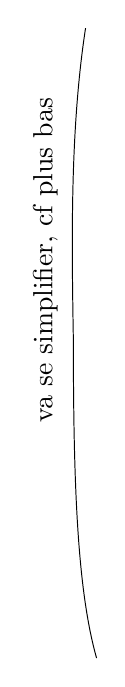
\begin{tikzpicture}[x=.5cm,y=.5cm]
\draw[line width=.35pt] (.25,7.9) .. controls (-.15,5.3) and (-.10,2.4) .. (-.06,0) .. controls (-.06,-3.8) and (.05,-6.4) .. (.53,-8.1);
\node[rotate=90,anchor=south,inner sep=2pt] at (-.30,2.0) {va se simplifier, cf plus bas};
\end{tikzpicture}}}

% @ upper middle, 2°)
2°) $F'\setminus G'\subset F\setminus G$ Soit $A'\in F'\setminus G'$, prouvons $A'\in F\setminus G$, et d'abord $A'\in F$. \deleted{On a} Soit $A$ le plus petit él. de $F^{A'}$ donc
% @ right end of this line: two inclusions over a bracket with raised end caps
% The two worked-over superscripts are retained separately; the far-right ending meets the paper edge.
\figure{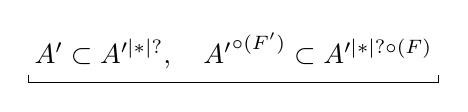
\begin{tikzpicture}
\node[inner sep=2pt] (formula) {$A'\subset A^{\deleted{\unsure{\prime|\ast|?}}},\quad {A'}^{\circ(F')}\subset A^{\deleted{\unsure{\prime|\ast|?}}\circ(\unsure{F)}}$};
\draw[line width=.6pt] (formula.south west) -- ([yshift=-.10cm]formula.south west) -- ([yshift=-.10cm]formula.south east) -- (formula.south east);
\end{tikzpicture}}
prouvons que $A'=A$ (d'où $A\in F$). \deleted{On a}

% @ middle, Je dis
Je dis que $A\in F\setminus G$ i.e. $A\notin G$, sinon on aurait $A\subset|G|=|G'|$ donc $A'\in G'$ puisque $A'\in F'$ et $G'\leq F'$, absurde. \deleted{Mais} Donc $A\in F\setminus G$, donc $A\in F'$, \deleted{\unsure{et}} Il en résulte que $A^{\circ(F)}=A^{\circ(F')}$ (car $F'\preceq F$\inserted{il suffirait $F'\ll F$}\deleted{)} cf lemme plus bas) et \uline{\unsure{bien}} \deleted{$\unsure{F|\in|\exists}$} $A,A'\in F'$ tels que ${A'}^{\circ(F')}\subset A^{\circ(F')}$, ce qui prouve $A=A'$.
% The short lower stroke at bien is read tentatively as an underline; cancellation remains possible.

% @ lower middle, Donc
Donc \unsure{on a} prouvé que $\deleted{\unsure{F|A}}A'\in F'\setminus G'\Rightarrow A'\in F$. Prouvons qu'on a $A'\notin G$ (d'où $A'\in F\setminus G$\deleted{)}, qed). Sinon on aurait $A'\in G$, on aurait $A'\subset |G|=|G'|$, d'où
% @ pale separate mark immediately above the final parenthetical line
% Arrow identification, function and hand uncertain; the visible shape is reproduced.
\figure{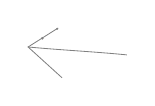
\begin{tikzpicture}[x=1cm,y=1cm,line cap=round]
\draw[gray,line width=.3pt] (1.25,0) .. controls (.85,.04) and (.43,.06) .. (0,.10);
\draw[gray,line width=.3pt] (.38,.34) -- (0,.10) -- (.43,-.29);
\fill[gray] (.18,.21) circle (.018);
\fill[gray] (.37,.33) circle (.014);
\end{tikzpicture}}
(comme $A'\in F'$ et $G'\leq F'$) $A'\in G'$, absurde.

% @ lower third, cancelled b) to c); all interlinear additions are within the cancellation
\deleted{b) $\Rightarrow$ c) \inserted{On suppose b) i.e. $\varphi$ induit $F'\setminus G'\overset{\sim}{\longrightarrow}F\setminus G$} Soit $A\in F\setminus G$, prouvons que $A^{\circ(F)}$ est une \uline{strate ouverte \deleted{dans \unsure{la}} de $F'$}. Soit $A'\in F'\setminus G'$ l'unique élément \deleted{de} tel que $\varphi(A')=A$. Prouvons ${A'}^{\circ(F')}=A^{\circ(F)}$.}

% @ bottom, b to c
b $\Longleftrightarrow$ c \deleted{Posons} On a $|F|\setminus|G|=|F'|\setminus|G'|$, soit $U$, Posons $F\setminus G=I^{\unsure{k|\ast|+}},\ F'\deleted{\unsure{\times|\setminus}}\unsure{\setminus}G'={I'}^{k}$ (parties ouvertes des ens d'indices ordonnés $\unsure{I|\vec I}$, \deleted{$A$} $(=F)$, $I'(=F')$. On a
% The forked superscript is the same ambiguous glyph in both I occurrences; k is the present ink preference.
% The top bar of the later I ends in an arrow-like hook; a separate arrow is not certain.
% No second closing parenthesis is visible at the end of the open parenthetical phrase.
